% Options for packages loaded elsewhere
\PassOptionsToPackage{unicode}{hyperref}
\PassOptionsToPackage{hyphens}{url}
%
\documentclass[
]{book}
\usepackage{amsmath,amssymb}
\usepackage{lmodern}
\usepackage{ifxetex,ifluatex}
\ifnum 0\ifxetex 1\fi\ifluatex 1\fi=0 % if pdftex
  \usepackage[T1]{fontenc}
  \usepackage[utf8]{inputenc}
  \usepackage{textcomp} % provide euro and other symbols
\else % if luatex or xetex
  \usepackage{unicode-math}
  \defaultfontfeatures{Scale=MatchLowercase}
  \defaultfontfeatures[\rmfamily]{Ligatures=TeX,Scale=1}
\fi
% Use upquote if available, for straight quotes in verbatim environments
\IfFileExists{upquote.sty}{\usepackage{upquote}}{}
\IfFileExists{microtype.sty}{% use microtype if available
  \usepackage[]{microtype}
  \UseMicrotypeSet[protrusion]{basicmath} % disable protrusion for tt fonts
}{}
\makeatletter
\@ifundefined{KOMAClassName}{% if non-KOMA class
  \IfFileExists{parskip.sty}{%
    \usepackage{parskip}
  }{% else
    \setlength{\parindent}{0pt}
    \setlength{\parskip}{6pt plus 2pt minus 1pt}}
}{% if KOMA class
  \KOMAoptions{parskip=half}}
\makeatother
\usepackage{xcolor}
\IfFileExists{xurl.sty}{\usepackage{xurl}}{} % add URL line breaks if available
\IfFileExists{bookmark.sty}{\usepackage{bookmark}}{\usepackage{hyperref}}
\hypersetup{
  pdftitle={Statistics Labs for Psychology},
  pdfauthor={Zakary A. Draper},
  hidelinks,
  pdfcreator={LaTeX via pandoc}}
\urlstyle{same} % disable monospaced font for URLs
\usepackage{color}
\usepackage{fancyvrb}
\newcommand{\VerbBar}{|}
\newcommand{\VERB}{\Verb[commandchars=\\\{\}]}
\DefineVerbatimEnvironment{Highlighting}{Verbatim}{commandchars=\\\{\}}
% Add ',fontsize=\small' for more characters per line
\usepackage{framed}
\definecolor{shadecolor}{RGB}{248,248,248}
\newenvironment{Shaded}{\begin{snugshade}}{\end{snugshade}}
\newcommand{\AlertTok}[1]{\textcolor[rgb]{0.94,0.16,0.16}{#1}}
\newcommand{\AnnotationTok}[1]{\textcolor[rgb]{0.56,0.35,0.01}{\textbf{\textit{#1}}}}
\newcommand{\AttributeTok}[1]{\textcolor[rgb]{0.77,0.63,0.00}{#1}}
\newcommand{\BaseNTok}[1]{\textcolor[rgb]{0.00,0.00,0.81}{#1}}
\newcommand{\BuiltInTok}[1]{#1}
\newcommand{\CharTok}[1]{\textcolor[rgb]{0.31,0.60,0.02}{#1}}
\newcommand{\CommentTok}[1]{\textcolor[rgb]{0.56,0.35,0.01}{\textit{#1}}}
\newcommand{\CommentVarTok}[1]{\textcolor[rgb]{0.56,0.35,0.01}{\textbf{\textit{#1}}}}
\newcommand{\ConstantTok}[1]{\textcolor[rgb]{0.00,0.00,0.00}{#1}}
\newcommand{\ControlFlowTok}[1]{\textcolor[rgb]{0.13,0.29,0.53}{\textbf{#1}}}
\newcommand{\DataTypeTok}[1]{\textcolor[rgb]{0.13,0.29,0.53}{#1}}
\newcommand{\DecValTok}[1]{\textcolor[rgb]{0.00,0.00,0.81}{#1}}
\newcommand{\DocumentationTok}[1]{\textcolor[rgb]{0.56,0.35,0.01}{\textbf{\textit{#1}}}}
\newcommand{\ErrorTok}[1]{\textcolor[rgb]{0.64,0.00,0.00}{\textbf{#1}}}
\newcommand{\ExtensionTok}[1]{#1}
\newcommand{\FloatTok}[1]{\textcolor[rgb]{0.00,0.00,0.81}{#1}}
\newcommand{\FunctionTok}[1]{\textcolor[rgb]{0.00,0.00,0.00}{#1}}
\newcommand{\ImportTok}[1]{#1}
\newcommand{\InformationTok}[1]{\textcolor[rgb]{0.56,0.35,0.01}{\textbf{\textit{#1}}}}
\newcommand{\KeywordTok}[1]{\textcolor[rgb]{0.13,0.29,0.53}{\textbf{#1}}}
\newcommand{\NormalTok}[1]{#1}
\newcommand{\OperatorTok}[1]{\textcolor[rgb]{0.81,0.36,0.00}{\textbf{#1}}}
\newcommand{\OtherTok}[1]{\textcolor[rgb]{0.56,0.35,0.01}{#1}}
\newcommand{\PreprocessorTok}[1]{\textcolor[rgb]{0.56,0.35,0.01}{\textit{#1}}}
\newcommand{\RegionMarkerTok}[1]{#1}
\newcommand{\SpecialCharTok}[1]{\textcolor[rgb]{0.00,0.00,0.00}{#1}}
\newcommand{\SpecialStringTok}[1]{\textcolor[rgb]{0.31,0.60,0.02}{#1}}
\newcommand{\StringTok}[1]{\textcolor[rgb]{0.31,0.60,0.02}{#1}}
\newcommand{\VariableTok}[1]{\textcolor[rgb]{0.00,0.00,0.00}{#1}}
\newcommand{\VerbatimStringTok}[1]{\textcolor[rgb]{0.31,0.60,0.02}{#1}}
\newcommand{\WarningTok}[1]{\textcolor[rgb]{0.56,0.35,0.01}{\textbf{\textit{#1}}}}
\usepackage{longtable,booktabs,array}
\usepackage{calc} % for calculating minipage widths
% Correct order of tables after \paragraph or \subparagraph
\usepackage{etoolbox}
\makeatletter
\patchcmd\longtable{\par}{\if@noskipsec\mbox{}\fi\par}{}{}
\makeatother
% Allow footnotes in longtable head/foot
\IfFileExists{footnotehyper.sty}{\usepackage{footnotehyper}}{\usepackage{footnote}}
\makesavenoteenv{longtable}
\usepackage{graphicx}
\makeatletter
\def\maxwidth{\ifdim\Gin@nat@width>\linewidth\linewidth\else\Gin@nat@width\fi}
\def\maxheight{\ifdim\Gin@nat@height>\textheight\textheight\else\Gin@nat@height\fi}
\makeatother
% Scale images if necessary, so that they will not overflow the page
% margins by default, and it is still possible to overwrite the defaults
% using explicit options in \includegraphics[width, height, ...]{}
\setkeys{Gin}{width=\maxwidth,height=\maxheight,keepaspectratio}
% Set default figure placement to htbp
\makeatletter
\def\fps@figure{htbp}
\makeatother
\setlength{\emergencystretch}{3em} % prevent overfull lines
\providecommand{\tightlist}{%
  \setlength{\itemsep}{0pt}\setlength{\parskip}{0pt}}
\setcounter{secnumdepth}{5}
\usepackage{booktabs}
\usepackage{amsthm}
\makeatletter
\def\thm@space@setup{%
  \thm@preskip=8pt plus 2pt minus 4pt
  \thm@postskip=\thm@preskip
}
\makeatother
\ifluatex
  \usepackage{selnolig}  % disable illegal ligatures
\fi
\usepackage[]{natbib}
\bibliographystyle{apalike}

\title{Statistics Labs for Psychology}
\author{Zakary A. Draper}
\date{2021-08-11}

\begin{document}
\maketitle

{
\setcounter{tocdepth}{1}
\tableofcontents
}
\hypertarget{authors-note}{%
\chapter*{Author's Note}\label{authors-note}}
\addcontentsline{toc}{chapter}{Author's Note}

Hi there. I hope you find this lab manual helpful. If you are an instructor who is interested in using these materials for your course, you can \href{mailto:zakary.draper@ubc.ca}{email me} and I can provide you with some additional resources.

\hypertarget{ost}{%
\chapter{\texorpdfstring{One Sample \emph{t} Tests}{One Sample t Tests}}\label{ost}}

One sample \emph{t} tests are conducted to test questions about the average value of a continuous variable in a population. For example, one-sample \emph{t} tests might be used to help answer the following research questions:

\begin{itemize}
\tightlist
\item
  Are Canadians aged 65 and older able to recall a 7-digit phone number?
\item
  Can university students type more than 60 words-per-minute?
\item
  Do North Americans consume 2000 calories per day?
\end{itemize}

Each of these research questions include a definition of a population, a variable measured on a continuous (or at least interval) scale, and a specific value on that scale. Note that there is no mention of how that value might compared with other populations. Research questions that can be informed by one-sample \emph{t} tests can always be framed in the form:

\begin{quote}
Is the average value of {[}continuous variable{]} among {[}characteristics of a population{]} {[}more than/less than/more or less than{]} exactly {[}a number{]}?
\end{quote}

One-sample \emph{t} tests are rarely used because most research questions cannot be phrased in this way. That's because of the ``{[}a number{]}'' part at the end. We are usually more interested in comparing values between populations (e.g., ``is the treatment more effective than a placebo?'') or in how a value changes based on some other continuous variable (e.g., ``does life satisfaction increase with age?'').

Although one-sample \emph{t} tests are rarely used, it is important to understand how they work. They are the simplest statistical models and the foundation of every other analysis covered in this lab. Mastering the one-sample \emph{t} test will prepare you for the more complex models that you will be building in future labs.

\hypertarget{ost-objectives}{%
\section{Learning Objectives}\label{ost-objectives}}

After completing this lab, you should be able to do the following using R:

\begin{itemize}
\tightlist
\item
  Conduct one-sample \emph{t} tests.
\item
  Compute Cohen's \emph{d}\textsubscript{z}.
\item
  Produce histograms.
\item
  Conduct Shapiro--Wilk tests.
\item
  Produce descriptive statistics including \emph{M}, \emph{SD}, skew, and kurtosis.
\end{itemize}

Additionally, you should be able to:

\begin{itemize}
\tightlist
\item
  Report results of one-sample \emph{t} tests in APA style.
\item
  Report results of Shapiro--Wilk tests in APA style.
\item
  Understand the role of the following in evaluating the strength of evidence provided by one-sample \emph{t} tests to support or refute hypotheses about a population:

  \begin{itemize}
  \tightlist
  \item
    The correct interpretation of a \emph{p} value.
  \item
    The assumption of normality in one-sample \emph{t} tests.
  \item
    Raw and standardized effect sizes.
  \end{itemize}
\end{itemize}

\hypertarget{ost-study}{%
\section{The Study: Is 7 Really Magical?}\label{ost-study}}

\emph{The following is the Introduction and Method sections of a hypothetical study. For this lab, you will conduct the analyses described in the analytic strategy below.}

Eminent psychologist George Miller is best known for his seminal paper, ``The Magical Number Seven, Plus or Minus Two: Some Limits on Our Capacity for Processing Information.'' ``The Magical Number Seven'' has been interpreted to claim that humans can hold an average of seven objects in working memory---an idea sometimes referred to as Miller's Law. Miller's Law proposes a remarkably simple model of working memory capacity. We tested this model of working memory in a sample of undergraduate psychology students who were in their third or later year of their program and had excelled in their coursework. Because these students had showcased academic excellence over several years of post-secondary education, we hypothesized that their memory spans would be greater than seven.

\hypertarget{participants-and-procedure}{%
\subsection*{Participants and Procedure}\label{participants-and-procedure}}
\addcontentsline{toc}{subsection}{Participants and Procedure}

Participants (\emph{N} = 174) were undergraduate psychology students enrolled in a research methods and statistics course designed to prepare students to conduct research and for graduate school. Entry into this course is competitive based on GPA in psychology courses. As such, these students were above average in terms of academic achievement. Participation in this study was part of the students' coursework.

\hypertarget{measures}{%
\subsection*{Measures}\label{measures}}
\addcontentsline{toc}{subsection}{Measures}

Memory span is the longest sequence of items a person is able to correctly repeat immediately after presentation, in at least 50\% of trials. We measured digit span, which is memory span for digits, using the R package memoryspan. This package includes a program for measuring digit span by printing digits to the R console and asking participants to type those values into the console. If the correct sequence of values is entered into the console, the user is presented with a new sequence which is one unit longer than the prior sequence. If the incorrect sequence is entered into the console, the trial ends and the user's digit span for that trial is returned. By default, the program begins with a digit span of one, but participants were instructed that they could increase this value to save time. Participants completed 10 trials. Their digit spans were defined as the longest sequence they correctly repeated in at least 5 of the 10 trials.

\hypertarget{analytic-strategy}{%
\subsection*{Analytic Strategy}\label{analytic-strategy}}
\addcontentsline{toc}{subsection}{Analytic Strategy}

To test whether Miller's Law applied to digit spans for this population of students, we conducted one-sample \emph{t} tests against the null hypothesis that our sample was drawn from a population in which average memory span is less than or equal to seven. One-sample t tests assume that variables are drawn from a normally distributed population. We tested this assumption by visually inspecting histograms, examining skew and kurtosis values, and with Shapiro--Wilk tests.

\hypertarget{ost-data-collection}{%
\section{Data Collection}\label{ost-data-collection}}

Use the R package \href{http://github.com/zakarydraper/MemorySpan}{\texttt{MemorySpan}} to complete 10 trials of a digit-span task. Record your results. Your digit span will be the longest list you correctly recall on at least 5 of the 10 trials. \texttt{MemorySpan} is not available on the CRAN. It can be installed from GitHub using the function \texttt{install\_github()} from the \texttt{remotes} package. Install \texttt{MemorySpan} by running \texttt{remotes::install\_github("zakarydraper/MemorySpan")}. As with R packages installed from the CRAN, this only needs to be installed once.

After installing \texttt{MemorySpan}, you can load it with \texttt{library()} like you would any other R package. Consult the documentation for \texttt{measure\_memory\_span()} for direction on how to use the function to measure your digit span.

\hypertarget{ost-assignment}{%
\section{Lab Report Instructions}\label{ost-assignment}}

Read ``Is 7 Really Magical? A Simple Test of Miller's Law,'' which is a manuscript containing an introduction and method section. For this lab, you will be conducting the analyses described in the analytic strategy (part of the method) and reporting the results in APA style. You will submit the following: (a) an R script for conducting the analyses described in the analytic strategy, (b) a Word document with your results reported in APA style, and (c) short answer responses to the discussion questions.

\hypertarget{r-script}{%
\subsection{R Script}\label{r-script}}

Do the following in R:

\begin{enumerate}
\def\labelenumi{\arabic{enumi}.}
\tightlist
\item
  Use \texttt{t.test()} to conduct a one-sample \emph{t} test of the null hypothesis that the average digit span in the population is less than or equal to 7. Use \texttt{\textless{}-} to assign a name to the output of your call to \texttt{t.test()}.
\item
  Compute Cohen's \emph{d}\textsubscript{z}, either by using the formula \((M - \mu)/SD\) or by converting from the \emph{t} with \texttt{psych::t2d()}.\footnote{The questions are identical to those used by \citet{davies2008} except ``Canadian'' replaces ``American'' in all instances.}
\item
  Use \texttt{hist()} to produce a histogram of the distribution of digit spans.
\item
  Use \texttt{shapiro.test()} to conduct a Shapiro--Wilk test on the distribution of digit spans.
\item
  Calculate \emph{M}, \emph{SD}, skewness, and kurtosis of the digit span variable. Calculate \emph{M}, \emph{SD}, and range of participant ages:

  \begin{itemize}
  \tightlist
  \item
    \texttt{psych::describe()} will calculate all of these values in one go.
  \item
    \texttt{QuantPsyc::norm()} will calculate skew and kurtosis for one variable and will provide significance tests for each (not provided with \texttt{psych::describe()}). It will not provide \emph{M}, \emph{SD}, or range.
  \end{itemize}
\end{enumerate}

\hypertarget{results}{%
\subsection{Results}\label{results}}

Your results section should include the following:

\begin{itemize}
\tightlist
\item
  1 sentence presenting the results of the one-sample \emph{t} test.
\item
  1 sentence presenting the results of the Shapiro--Wilk test.
\item
  1--3 sentences describing the distribution of scores. Reference the results of the Shapiro--Wilk test, the histogram (i.e., Figure 1 in your manuscript), and skew and kurtosis values.
\item
  A histogram showing the distribution of digit spans in the sample. Follow the rules for figures in the \emph{APA Publication Manual}.
\end{itemize}

\hypertarget{discussion}{%
\subsection{Discussion}\label{discussion}}

In future lab reports, you will write complete (albeit brief) discussion sections. For this lab report, answer each of the following questions in complete sentences.

\begin{itemize}
\tightlist
\item
  Do your results support your hypothesis?
\item
  How do your results compare with Miller's work arguing that memory span is equal to seven? Provide an explanation for why your results agree or disagree.
\item
  How does the characteristics of the sample affect your interpretation of these results?
\item
  What is an implication of your findings for future research, programs, or policy?
\end{itemize}

\hypertarget{pst}{%
\chapter{\texorpdfstring{Paired Samples \emph{t} Tests}{Paired Samples t Tests}}\label{pst}}

Last lab covered one sample \emph{t} tests. We learned that one sample \emph{t} tests compare the mean to a specific value. One common use case for this is when pairs of scores can be represented using a single value. For example, imagine you want to test whether cognitive behavioural therapy (CBT) reduces generalized anxiety. Study participants could complete the GAD-7 (a popular measure of generalized anxiety) prior to receiving treatment. Then, after receiving CBT, they could be take the GAD-7 again. The resulting data would be two GAD-7 scores for each participant. If we want to know whether a participant's anxiety decreased, increased, or stayed the same, we could just subtract their pre-treatment score from their post-treatment score. Doing this for each participant yields a single variable that represents the difference (or change) from pre- to post-treatment. We could then conduct a one sample \emph{t} test on the change scores.

Another name for this procedure is a paired samples \emph{t} test. It is so named because the data are two samples that are \emph{paired}. In the example above, samples are paired because they come from the same participant measured on two occasions. This is likely the most common design that leads to paired samples. However, pairs of observations can also come from different individuals. For example, if you wanted to know whether birth influences language acquisition, you could compare the number of words a firstborn child knew at 12 months to the number of words a second born child from the same family knew at 12 months. In this case observations are paired because they come from the same family.

If you are wondering whether a paired samples \emph{t} test is appropriate for your research design, ask yourself whether it makes sense to produce difference scores for your cases. Note that difference scores are not valid when pairs of observations are measured in different metrics. If a pre-to-post design (such as in the CBT example above) uses a different measurement instrument at each measurement occasion (even if both instruments are intended to measure the same construct), difference scores are no longer valid. Another situation when difference scores won't work is when groups of observations are dependent, but not paired. For example, if the CBT study above included participants from several different therapists. Participants with the same therapist would be expected to be more similar to one another than to participants from different therapists. But a paired samples \emph{t} test could not be used to compare them because each participant is not matched to a single other participant.

Because paired samples \emph{t} tests are so similar (mathematically identical, even!) to one sample \emph{t} tests, this lab will give you an opportunity to polish the skills you have already learned. It will also introduce to the important considerations that are unique to paired samples.

\hypertarget{pst-learning-objectives}{%
\section{Learning Objectives}\label{pst-learning-objectives}}

After completing this lab, you should be able to do the following using R:

\begin{itemize}
\tightlist
\item
  Conduct paired samples \emph{t} tests.
\item
  Compute Cohen's \emph{d}\textsubscript{z} for paired samples.
\item
  Create appropriate visualizations for comparisons of two paired samples.
\end{itemize}

Additionally, you should be able to:

\begin{itemize}
\tightlist
\item
  Explain how paired samples \emph{t} tests are similar (and distinct) from one sample \emph{t} tests.
\item
  Evaluate the assumptions of paired samples \emph{t} tests.
\item
  Accurately interpret the results of paired samples \emph{t} tests.
\item
  Report the results of paired samples \emph{t} tests in APA style.
\end{itemize}

\hypertarget{pst-study}{%
\section{The Study: Weight-Loss-Related Self-Efficacy}\label{pst-study}}

\hypertarget{study-information}{%
\subsection{Study Information}\label{study-information}}

\hypertarget{description}{%
\subsubsection{Description}\label{description}}

Weight-loss interventions aim to support people in changing their behaviours to be healthier. This includes promoting healthy-eating and exercise. Self-efficacy is thought to be important for adopting and maintaining such behaviours. That is, people will change their behaviours if they believe they can maintain those behaviours and if they believe that changing their behaviour will help them lose weight.

Because self-efficacy is so important to the success of weight-loss interventions, some such interventions now include psychotherapy specifically aimed at improving self-efficacy. Weight-loss interventions provide instrumental support in helping participants develop a plan for eating healthful foods and engaging in regular physical activity. This has a clear and obvious benefit for self-efficacy. The current study will examine how subsequent psychotherapy further boosts self-efficacy.

\hypertarget{hypothesis}{%
\subsubsection{Hypothesis}\label{hypothesis}}

The primary hypothesis is that adding psychotherapy to a weight-loss intervention will lead to increased weight-loss self-efficacy.

\hypertarget{design-plan}{%
\subsection{Design Plan}\label{design-plan}}

\hypertarget{study-design}{%
\subsubsection{Study Design}\label{study-design}}

This study will use a within-subjects (paired) design. Participants will be enrolled in a weight-loss intervention at UBCO. They will attend a group session where they are provided general information about healthy eating, and physical activity. They will then have one-on-one interviews with a nutritionist to help them build meal plans that fit their budgets and lifestyles. Following the interviews, the nutritionist will ask participants to complete measures of weight-loss self-efficacy (WLSE). Participants will then meet with a trained psychotherapist who will work with the participants to identify potential barriers to their success and develop strategies for overcoming those barriers. After psychotherapy, participants will be asked to complete the same measure of WLSE.

\hypertarget{measures-1}{%
\subsubsection{Measures}\label{measures-1}}

Weight-loss-related behaviour self-efficacy will be measured using the scale proposed by \citet{wlse}. This scale has four items, measured on an 11-point scale ranging from 0\% (\emph{Not at All Confident}) to 100\% (\emph{Completely Confident}). The scale is relatively new; however, it has demonstrated strong psychometric properties in a large sample drawn from a population that is similar to the population used in the current study \citep{wlse}.

\hypertarget{analytic-strategy-1}{%
\subsubsection{Analytic Strategy}\label{analytic-strategy-1}}

We will conduct a directional paired samples \emph{t} test of the null hypothesis that average change in WLSE in the population is equal to zero. Significance will be based on the traditional α = .05.

\hypertarget{sample-size-and-power-analysis}{%
\subsubsection{Sample Size and Power Analysis}\label{sample-size-and-power-analysis}}

We want to be able to detect a difference of 10 points on the WLSE measure. This measure had a \emph{SD} = 21.44 in a large sample from a similar population \citep{wlse}. Assuming the same \emph{SD} in our sample, a 10-point change translates to Cohen's \emph{d}\textsubscript{z} = 0.47. To achieve 95\% power with a population effect of that size requires a sample of \emph{N} = 50.4. We are therefore aiming for a sample of \emph{N} = 51.

\hypertarget{pst-data}{%
\section{Data Collection}\label{pst-data}}

How confident are you that you can \textbf{lose weight\ldots{}}

\ldots even if you need a long time to develop the necessary routines?

(Select an Option)
0\% (Not at all Confident)
10\%
20\%
30\%
40\%
50\%
60\%
70\%
80\%
90\%
100\% (Completely Confident)

\ldots even if you have to try several times before it works?

(Select an Option)
0\% (Not at all Confident)
10\%
20\%
30\%
40\%
50\%
60\%
70\%
80\%
90\%
100\% (Completely Confident)

\ldots even if you have to rethink your entire way of losing weight?

(Select an Option)
0\% (Not at all Confident)
10\%
20\%
30\%
40\%
50\%
60\%
70\%
80\%
90\%
100\% (Completely Confident)

\ldots even if you have to make a detailed plan?

(Select an Option)
0\% (Not at all Confident)
10\%
20\%
30\%
40\%
50\%
60\%
70\%
80\%
90\%
100\% (Completely Confident)

\hypertarget{pst-assignment}{%
\section{Assignment Instructions}\label{pst-assignment}}

\hypertarget{r-script-1}{%
\subsection{R Script}\label{r-script-1}}

\begin{enumerate}
\def\labelenumi{\arabic{enumi}.}
\tightlist
\item
  Calculate participants' mean scores on the 5-item WLSE measure. Do this separately for the two measurement occasions. See the {[}additional instructions on scoring{]}{[}pst-scoring{]}.
\item
  Calculate \emph{M} and \emph{SD} for the pre- and post-psychotherapy means, and \emph{M}, \emph{SD}, skew, and kurtosis of the difference scores.
\item
  Use \texttt{t.test()} to conduct a paired \emph{t} test of the null hypothesis that average pre-to-post change in WLSE scores is zero.
\item
  Compute Cohen's \emph{d}\textsubscript{z} for the change in WLSE scores.
\item
  Produce a histogram of the WLSE difference scores.
\item
  Conduct a Shapiro--Wilk test on the difference scores.
\item
  Produce a boxplot of pre- and post-psychotherapy WLSE scores. See the {[}additional instructions{]}{[}pst-plotting{]} below.
\end{enumerate}

\hypertarget{pst-additional-instructions}{%
\subsection{Additional Instructions}\label{pst-additional-instructions}}

\hypertarget{pst-scoring}{%
\subsubsection{Scoring}\label{pst-scoring}}

The ``weight-loss.csv'' data frame includes item-level data. That is, each column is one item on the WLSE measure. Use \texttt{rowMeans()} to calculate each participant's average score on the 5-item measure. Do this separately for the time 1 and time 2 measurement occasions. Add participants' mean scores on times 1 and 2 as columns to your data frame.

Calculate difference/change scores for each participant. This will be the difference between each participant's average WLSE scores at times 1 and 2. When computing difference scores, it is conventional to subtract initial scores from final scores (i.e., time 2 − time 1). Doing this makes the difference scores more interpretable, as a negative difference score means a decrease, and a positive score means an increase.

\hypertarget{descriptive-statistics}{%
\subsubsection{Descriptive Statistics}\label{descriptive-statistics}}

Produce the following statistics:

\begin{itemize}
\tightlist
\item
  \emph{M} and \emph{SD} of average WLSE scores at both measurement occasions.
\item
  \emph{M}, \emph{SD}, skew, kurtosis of the difference scores.
\end{itemize}

\hypertarget{paired-t-test}{%
\subsubsection{\texorpdfstring{Paired \emph{t} Test}{Paired t Test}}\label{paired-t-test}}

Use \texttt{t.test()} to conduct a directional paired samples \emph{t} test comparing WLSE scores before and after psychotherapy.

Use \texttt{t.test()} to conduct a one sample \emph{t} test on the difference scores. What do you notice about the results of this test and the results of the paired \emph{t} test?

\hypertarget{cohens-dz}{%
\subsubsection{\texorpdfstring{Cohen's \emph{d}\textsubscript{z}}{Cohen's dz}}\label{cohens-dz}}

Calculate Cohen's \emph{d}\textsubscript{z} either by converting \emph{t} to \emph{d} using \texttt{psych::t2d()}, or using the \emph{M} and \emph{SD} of the difference scores in the formula \(d_{z} = M/SD\).\footnote{The questions are identical to those used by \citet{davies2008} except ``Canadian'' replaces ``American'' in all instances.}

\hypertarget{pst-plotting}{%
\subsection{Plots}\label{pst-plotting}}

This section will guide you through the process of producing a figure like the one below.

\begin{figure}
\centering
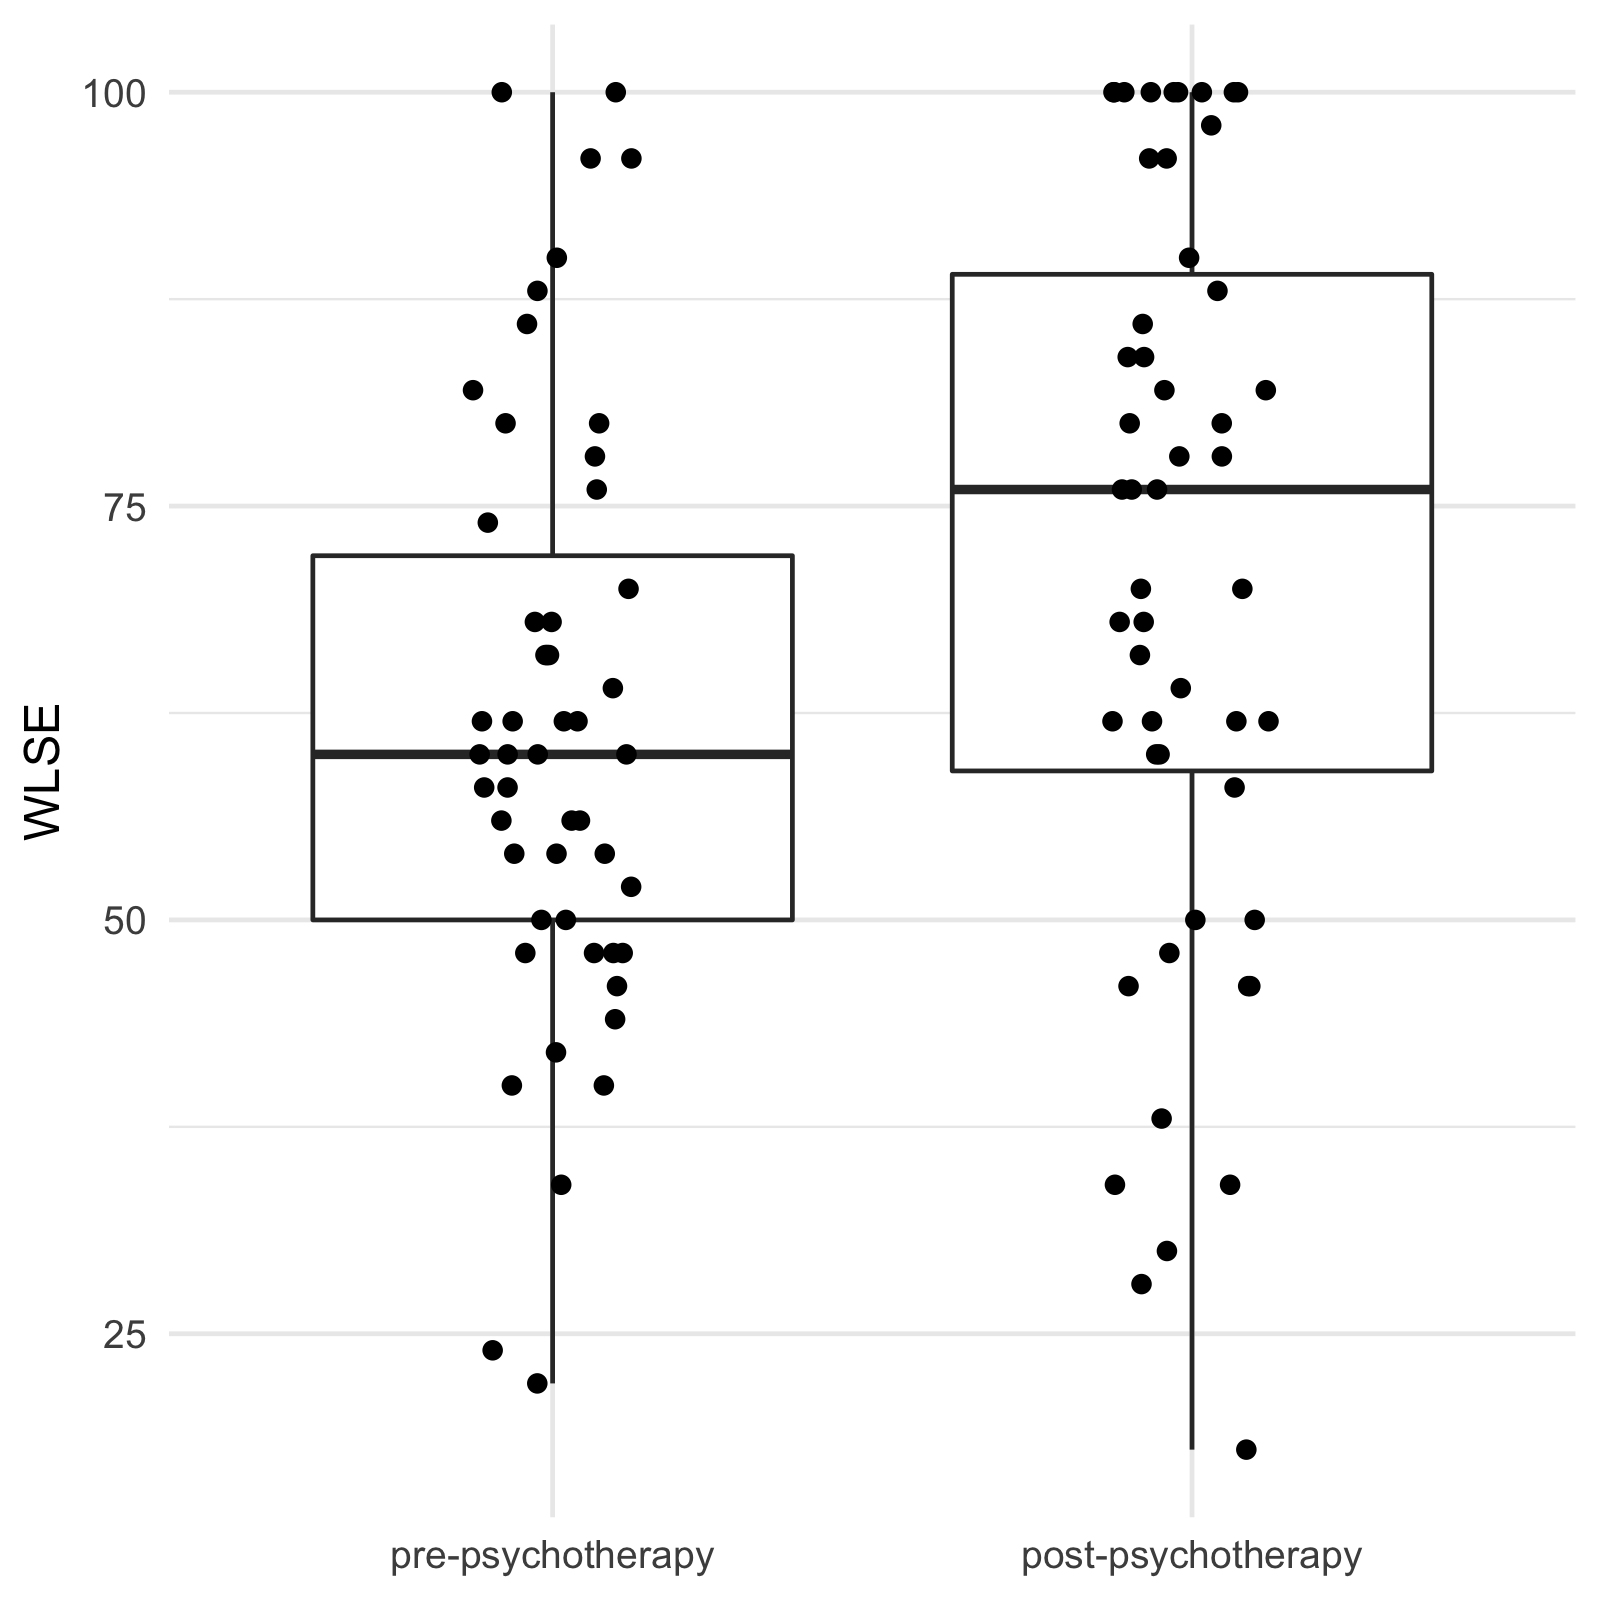
\includegraphics{img/wlse-boxplot.png}
\caption{boxplot}
\end{figure}

This is a boxplot with individual data points overlaid. It is a very useful plot because it concisely presents a lot of information.

\hypertarget{lengthen-the-data}{%
\subsubsection{Lengthen the Data}\label{lengthen-the-data}}

The data are currently arrange such that scores at each measurement occasion are placed in their own columns. That is, there are separate columns for time 1 and time 2 scores.

\begin{longtable}[]{@{}ccc@{}}
\toprule
pid & wlse\_m.t1 & wlse\_m.t2 \\
\midrule
\endhead
1 & 44 & 50 \\
2 & 78 & 62 \\
3 & 96 & 84 \\
\bottomrule
\end{longtable}

The same data could be arranged with a single column for each item, and an additional column indicating whether the responses are for time 1 or time 2. That is, instead of time 1 and time 2 responses being differentiated by column, they are differentiated by row.

\begin{longtable}[]{@{}ccc@{}}
\toprule
pid & name & value \\
\midrule
\endhead
1 & wlse\_m.t1 & 44 \\
1 & wlse\_m.t2 & 50 \\
2 & wlse\_m.t1 & 78 \\
2 & wlse\_m.t2 & 62 \\
3 & wlse\_m.t1 & 96 \\
3 & wlse\_m.t2 & 84 \\
\bottomrule
\end{longtable}

Neither of these two options are strictly better than the other. The way the data should be arranged depends on what you are doing with the data. The wider format we have used so far has made sense for what we have been doing. For example, think about how difficult it would be to calculate changer scores if the data were arranged in this longer format.

That said, the plot we want to produce has time on the x axis, and scores on the y axis. To create this plot, time needs its own column in the data frame. So, even though the wider format has made sense so far, we'll need to pivot to the longer format in order to make the plot.

There are many options for reshaping data frames. The easiest (and it isn't close) is to use \texttt{tidyr::pivot\_longer()} and \texttt{tidyr::pivot\_wider()}. For a detailed introduction to these functions, see \href{https://r4ds.had.co.nz/tidy-data.html}{Chapter 12 of R for Data Science}.

\texttt{tidyr::pivot\_longer()} has many arguments, but most are optional. You can lengthen your data frame using just the first two arguments: \texttt{data} and \texttt{cols}. The first argument, \texttt{data}, is the data frame you want to lengthen. The second argument, \texttt{cols}, is the names of the variables in that data frame that should be pivoted into the longer format.

Two optional arguments you may find useful are \texttt{names\_to} and \texttt{values\_to}. These can be used to specify the names of the new columns in the longer data frame. For example, I've renamed my name column ``time,'' and my value column ``wlse.''

\begin{longtable}[]{@{}ccc@{}}
\toprule
pid & time & wlse \\
\midrule
\endhead
1 & wlse\_m.t1 & 44 \\
1 & wlse\_m.t2 & 50 \\
2 & wlse\_m.t1 & 78 \\
2 & wlse\_m.t2 & 62 \\
3 & wlse\_m.t1 & 96 \\
3 & wlse\_m.t2 & 84 \\
\bottomrule
\end{longtable}

You'll notice that the pivoted data frame looks different than the data frames you have seen thus far. It prints \texttt{\#A\ tibble:} and the number of rows and columns. It also gives the data types of the columns in the data frame. That's because the output of \texttt{tidyr::pivot\_longer()} (and the related function \texttt{tidyr::pivot\_wider()}) is not a \texttt{data.frame}, but a \texttt{tibble}. A \texttt{tibble} is a variant of a \texttt{data.frame} and functions in much the same way. For more information on tibbles, see \href{https://r4ds.had.co.nz/tibbles.html}{Chapter 10 of R for Data Science}. If you want to turn your \texttt{tibble} back into a \texttt{data.frame}, use \texttt{as.data.frame()}.

Let's turn our attention to the \texttt{time} column. This is a character vector. That means that the values in \texttt{time} are unordered. But the values represent an ordered variable (i.e., t1 comes before t2). Also, the values are kind of ugly. In the next step, we'll be plotting these values, and we don't want these ugly names showing up as labels on our plots. We can solve both these problems by converting this character vector to a factor using \texttt{factor()}.

\begin{longtable}[]{@{}ccc@{}}
\toprule
pid & time & wlse \\
\midrule
\endhead
1 & pre-psychotherapy & 44 \\
1 & post-psychotherapy & 50 \\
2 & pre-psychotherapy & 78 \\
2 & post-psychotherapy & 62 \\
3 & pre-psychotherapy & 96 \\
3 & post-psychotherapy & 84 \\
\bottomrule
\end{longtable}

\hypertarget{produce-the-plot}{%
\subsubsection{Produce the Plot}\label{produce-the-plot}}

With the data frame lengthened, you are now ready to produce the boxplot.

\hypertarget{ist}{%
\chapter{\texorpdfstring{Independent Samples \emph{t} Tests}{Independent Samples t Tests}}\label{ist}}

\hypertarget{ist-learning-objectives}{%
\section{Learning Objectives}\label{ist-learning-objectives}}

After completing this lab, you should be able to do the following using R:

\begin{itemize}
\tightlist
\item
  Conduct both Student's and Welch's independent samples \emph{t} tests.
\item
  Compute Cohen's \emph{d} by conversion from the test statistic using \texttt{psych::t2d()} or by computing Cohen's \emph{d} directly using \texttt{psych::cohen.d()}.
\item
  Create appropriate visualizations for comparisons of two independent samples (as described in the assignment instructions).
\item
  Produce a single figure with plots for each level of a grouping variable using \texttt{ggplot2::facet\_wrap()}.
\item
  Calculate group-level descriptive statistics using \texttt{describeBy()}.
\end{itemize}

Additionally, you should be able to:

\begin{itemize}
\tightlist
\item
  Evaluate the assumptions of independent samples \emph{t} tests.
\item
  Explain the difference between Student's \emph{t} tests and Welch's \emph{t} tests.
\item
  Accurately interpret the results of independent samples \emph{t} tests.
\item
  Report the results of independent samples \emph{t} tests in APA style.
\end{itemize}

\hypertarget{ist-study}{%
\section{The Study: Social Identity}\label{ist-study}}

\hypertarget{study-information-1}{%
\subsection{Study Information}\label{study-information-1}}

\hypertarget{description-1}{%
\subsubsection{Description}\label{description-1}}

People desire positive social identities. A positive social identity is achieved when the social groups to which one belongs (i.e., the ``ingroups'') are perceived as favourable to the social groups to which they do not belong (i.e., the ``outgroups''). Such positive social identities are most often fostered by favouring ingroup members, rather than by devaluing outgroups. As such, people tend to feel positively towards those they see as part of their ingroup.

The desire for a positive social identity can lead to discrimination when positive feelings are reserved for one's ingroup. However it can also promote acceptance of diversity. Preserving positive social identities requires accepting diversity within one's social groups. As such, broadly defining one's ingroup can foster a greater acceptance of diversity. Therefore, encouraging the adoption of broad social groups has been proposed as a means of combatting discrimination.

Of course changing how people define their ingroup is difficult. It can occur when one changes social groups, such as when one moves to a new community, makes new friends, or changes political parties. More often however, broadening one's ingroup is accomplished by strengthening ties with existing groups. That is, rather than changing the social groups to which they belong, people are more likely to change which social groups they see as important to their social identities.

This study will examine one mechanism by which people determine the importance of social groups to their social identities: perceived social group threat. Research has demonstrated that people strengthen ties to social groups when they perceive those groups as threatened in some way. This was evident in the aftermath of the 9/11 attacks on the United States. Many US citizens felt a threat to their American social identity. This led to a dramatic outpouring of displays of patriotism, such as flying the US flag on one's property.

Research conducted in the time after the 9/11 attacks revealed that one impact of this increased patriotism was a a greater tolerance for domestic multiculturalism. That is, people who felt a threat to their American social identity, were more accepting of diversity among American citizens.

One study conducted in that time utilized an experimental manipulation wherein some participants were introduced to a threat American social identity prior to being asked their agreement with statements related to American multiculturalism \citep{davies2008}. This study will investigate a similar effect using a Canadian sample. Although Canada and United States are similar in many ways, their political climates are distinct. Additionally, the political climate in Canada and the United States has changed in the years since this research was conducted. Political convictions are more rigid than they were. These factors could mean that the effects observed among Americans in 2001 will be different than what can be expected among Canadians today.

\hypertarget{hypothesis-1}{%
\subsubsection{Hypothesis}\label{hypothesis-1}}

It is expected that Canadians who are primed to perceive a threat to Canadian social identity, will be more accepting of multiculturalism in Canada.

\hypertarget{design-plan-1}{%
\subsection{Design Plan}\label{design-plan-1}}

\hypertarget{study-design-1}{%
\subsubsection{Study Design}\label{study-design-1}}

This study will employ an experimental design adapted from experiment 3 of \citet{davies2008}. Participants will read a brief newspaper article describing either a foreign or domestic event that could be perceived as threatening to Canadians. They will then complete a measure of national identity. Participants will be recruited at in-person public events throughout the Okanagan during the summer of 2021. Research assistants will operate tables at events throughout the summer. For completing the study, participants will be offered \$5.00 food vouchers redeemable at participating vendors at the event. Recruitment will continue until sufficient data are obtained or until the summer's end.

Individuals must be at least 18-years-old and Canadian citizens to be eligible to participate.

\hypertarget{measures-2}{%
\subsubsection{Measures}\label{measures-2}}

National identity will be measured with items adapted\footnote{The questions are identical to those used by \citet{davies2008} except ``Canadian'' replaces ``American'' in all instances.} from \citet{davies2008}. They will be measured on a 7-point Likert-type scale ranging from 1 (\emph{not at all}) to 7 (\emph{completely}).

\begin{enumerate}
\def\labelenumi{\arabic{enumi}.}
\tightlist
\item
  Do you identify with being Canadian?
\item
  Is being Canadian important to you?
\item
  Are you proud to be a Canadian?
\item
  Do you think of yourself as a Canadian?
\end{enumerate}

Participant scores will be averaged across these four items to create a composite measure of national identity.

\hypertarget{analytic-strategy-2}{%
\subsubsection{Analytic Strategy}\label{analytic-strategy-2}}

A directional Welch's \emph{t} test will be conducted with the alternative hypothesis that national identity is higher in the foreign threat condition. Significance will be inferred using the traditional α = .05.

\hypertarget{sample-size-and-power-analysis-1}{%
\subsubsection{Sample Size and Power Analysis}\label{sample-size-and-power-analysis-1}}

We plan to recruit 254 participants divided evenly into the two experimental conditions. This will provide 95\% power to detect an effect if the effect size in the population is \emph{d} = 0.414.

\citet{davies2008} reported mean national identities of 5.57 and 4.99 for participants who read about foreign and domestic threats, respectively. This amounts to a raw difference of 0.58 on the scale of 1 to 7. Because the \emph{SD}s for national identity were not reported, we cannot know the standardized effect size for this effect. We therefore based our effect size calculation on an assumed pooled \emph{SD} of 1.4. Under this assumption, a raw effect of 0.58 translates to \emph{d} = 0.414.

\hypertarget{ist-assignment}{%
\section{Assignment Instructions}\label{ist-assignment}}

Prepare an R script and written report presenting the results of the analysis described in the analytic strategy.

\hypertarget{r-script-2}{%
\subsection{R Script}\label{r-script-2}}

Your R script should be reproducible and free of errors. It should contain syntax to do the following:

\begin{itemize}
\tightlist
\item
  Import the data and convert the ``condition'' variable to a factor.
\item
  Calculate participant mean scores on the 4-item national identity measure.
\item
  Compute descriptive statistics, including \emph{M}, \emph{SD}, skew, and kurtosis of participants' mean national identity. Do this separately for each level of the experimental manipulation. Use \texttt{psych::describeBy()} to do this in a single step.
\item
  Conduct Shapiro--Wilk tests of normality for the distributions of national identity in each of the two conditions.
\item
  Compute a Welch's \emph{t} test as described in the analytic strategy.
\item
  Calculate the corresponding Cohen's \emph{d} effect size for the \emph{t} test.
\end{itemize}

\hypertarget{r-script-detailed-instructions}{%
\subsection{R Script (Detailed Instructions)}\label{r-script-detailed-instructions}}

\hypertarget{doing-a-t-test}{%
\subsubsection{\texorpdfstring{Doing a \emph{t} Test}{Doing a t Test}}\label{doing-a-t-test}}

There are two syntax options for conducting independent samples \emph{t} tests using \texttt{t.test()}. The first is similar the syntax used for the paired samples \emph{t} test. This involves supplying a numeric vector to the arguments \texttt{x} and \texttt{y}, which are the first two arguments of \texttt{t.test()}. A paired samples \emph{t} test requires the additional argument \texttt{paired\ =\ TRUE}. To indicate that the samples are independent, the argument should be \texttt{paired\ =\ FALSE}. The default value is already \texttt{paired\ =\ FALSE} so not specifying the argument will treat the samples as independent.

So, if I have a \texttt{data.frame} called \texttt{dta} that looks like this:

\begin{verbatim}
##   var1 var2
## 1    7   10
## 2    8    3
## 3    5    2
## 4    7    3
## 5    3    4
\end{verbatim}

Then I could conduct a \emph{t} test using the following syntax:

\begin{Shaded}
\begin{Highlighting}[]
\FunctionTok{t.test}\NormalTok{(}\AttributeTok{x =}\NormalTok{ dta}\SpecialCharTok{$}\NormalTok{var1, }\AttributeTok{y =}\NormalTok{ dta}\SpecialCharTok{$}\NormalTok{var2)}
\end{Highlighting}
\end{Shaded}

This would conduct what is called a Welch's \emph{t} test, which I explain below. When you inspected your data, you probably noticed that it is not arranged as the data above. Your data are arranged in a \texttt{data.frame} like this:

\begin{verbatim}
##    var value
## 1    1     7
## 2    1     8
## 3    1     3
## 4    1     4
## 5    1     9
## 6    2     4
## 7    2     7
## 8    2     1
## 9    2     8
## 10   2     2
\end{verbatim}

This is probably the most sensible way to arrange data from independent samples. It places observations from different people on separate rows. The prior arrangement had data from different people in different columns. That arrangment implies some connection between data from the same row, when there is none. It technically works when there are only two variables, but that is never the case with real data. You are going to have other information, such as participant IDs, demographic details, and so on that are unique to each participant. There is no sensible way of arranging the data frame that maintains the information about individual participants while placing scores from different participants side-by-side.

So, how do we make this second layout work with \texttt{t.test()}? There are two approaches. The first is to use \texttt{subset()}.

\begin{Shaded}
\begin{Highlighting}[]
\FunctionTok{t.test}\NormalTok{(}
  \AttributeTok{x =} \FunctionTok{subset}\NormalTok{(dta, var }\SpecialCharTok{==} \DecValTok{1}\NormalTok{)}\SpecialCharTok{$}\NormalTok{value,}
  \AttributeTok{y =} \FunctionTok{subset}\NormalTok{(dta, var }\SpecialCharTok{==} \DecValTok{2}\NormalTok{)}\SpecialCharTok{$}\NormalTok{value}
\NormalTok{)}
\end{Highlighting}
\end{Shaded}

This works, but there is another (in my opinion more elegant) approach as well. This is using the formula notation.

\hypertarget{formula-notation}{%
\subsubsection{Formula Notation}\label{formula-notation}}

Instead of passing values to \texttt{x} and \texttt{y}, you can specify a formula and a data frame.

\begin{Shaded}
\begin{Highlighting}[]
\FunctionTok{t.test}\NormalTok{(}\AttributeTok{formula =}\NormalTok{ value }\SpecialCharTok{\textasciitilde{}}\NormalTok{ var, }\AttributeTok{data =}\NormalTok{ dta)}
\end{Highlighting}
\end{Shaded}

This is telling \texttt{t.test()} to predict the values of \texttt{value} from the levels of \texttt{var}. Note that this does not use the \texttt{\$} to extract the values from the data frame. Instead, the \texttt{data} argument tells \texttt{t.test()} where the columns in the formula can be found. Formula notation will continue to show up throughout the course. It always follows the format \texttt{outcome\ \textasciitilde{}\ predictors}. The \texttt{\textasciitilde{}} (called ``tilda'') is on your keyboard above the ``tab'' key. In the context of formula notation it means ``is predicted from.'' In the context of a \emph{t} test, the outcome variable must be numeric and the predictor variable must have only two levels. The \texttt{t.test()} function will return an error if either of those things are untrue.

You can then pass additional values to arguments of \texttt{t.test()}, such as to \texttt{alternative}, \texttt{paired}, and \texttt{conf.level}.

\hypertarget{welchs-t-test}{%
\subsubsection{\texorpdfstring{Welch's \emph{t} Test}{Welch's t Test}}\label{welchs-t-test}}

The above examples have all done a Welch's \emph{t} test. Welch's \emph{t} test is the same as a regular \emph{t} test except that it includes an adjustment for the degrees of freedom. One of the assumptions of \emph{t} tests is equal variance in each of the two samples. This assumption is often not met. For example, in the example you are working on for your assignment, it could be that participants who read about a foreign threat responded more similarly to one another than participants who read about a domestic threat. This would violate the assumption of homogeneity of variance, meaning that the regular \emph{t} test would not be valid. Welch's \emph{t} test adjusts the degrees of freedom based on the degree of heterogenity of variance between the two samples. This will make the \emph{p} value larger but it means that you don't need to assume homogeneity of variance for the test to be valid.

If there is no heterogeneity of variance between the samples, Welch's \emph{t} test will produce the same result as a regular \emph{t} test. As such, it makes sense to just use Welch's \emph{t} test all the time. It removes an assumption and only affects the \emph{p} value when necessary. The author of \texttt{t.test()} agrees with this assessment and has therefore made the default independent samples \emph{t} test a Welch's \emph{t} test. If you want to conduct a traditional \emph{t} test, you must specify that using \texttt{var.equal\ =\ TRUE}. This means you are assuming equal variances in the two samples. I don't recommend ever doing this for your own research. However, you are likely to encounter regular \emph{t} tests in other people's work. If you want to reproduce their results, you will need to use this argument.

\hypertarget{describeby}{%
\subsubsection{describeBy()}\label{describeby}}

\hypertarget{manuscript}{%
\subsection{Manuscript}\label{manuscript}}

Prepare a written document that includes a one-paragraph description of the results and a one-paragraph discussion. The manuscript should follow the \href{https://apastyle.apa.org/jars/quantitative}{APA Journal Article Resporting Standards for Quantitative Research (JARS--Quant)}. Note that these guidelines are broad and ask for more information than required for the purpose of this lab report. You need not report information about dates of recruitment and data collection or missing data (though this information would be reported if it were a real study!).

The results section should include the following:

\begin{itemize}
\tightlist
\item
  Total participants in each experimental condition (note that the actual number of participants might differ from the planned number of participants in the study preregistration).
\item
  \emph{M} and \emph{SD} of national identity for each experimental group.
\item
  Results of the null-hypothesis significance test and corresponding standardized effect size.
\item
  Description of your efforts to diagnose problems with statistical assumptions and data distributions.
\item
  A figure visualizing mean national identity in each of the two groups and error associated with that measurement. The figure should be referenced in the text of the results section.
\end{itemize}

The discussion section should adhere to the \href{https://apastyle.apa.org/jars/quantitative}{JARS--Quant} guidelines. You can use these questions as a guide.

\begin{itemize}
\tightlist
\item
  Was the hypothesis supported? 1 sentence.
\item
  How do your results compare to the results reported by \citet{davies2008}? Consider both the size of the effect and the results of the significance test. 1--2 sentences.
\item
  Why do you think the results do or do not support the hypothesis? Consider both substantive theoretical reasons as well as design and statistical considerations.
\item
  Canadian adults are the implied population of interest in this study. Given the sampling design, how well does this sample represent that population? How does that affect the interpretation of these results? 2--3 sentences.
\item
  The broad theoretical mechanism under study was one in which the perception of an external threat to a social group leads to increased identification with that social group. In what contexts does this study have implications for this theory? Consider how the study's design might limit its generalizability. 1--3 sentences.
\item
  What is an implication of this research for future research, programs, or policy? 1--2 sentences.
\end{itemize}

\hypertarget{cor}{%
\chapter{Correlation}\label{cor}}

This lab will cover how to test hypotheses about the associations between two continuous variables.

\hypertarget{cor-learning-objectives}{%
\section{Learning Objectives}\label{cor-learning-objectives}}

\hypertarget{cor-study}{%
\section{The Study:}\label{cor-study}}

\hypertarget{cor-data}{%
\section{Data Collection}\label{cor-data}}

\hypertarget{cor-assignment}{%
\section{Assignment Instructions}\label{cor-assignment}}

\hypertarget{mreg}{%
\chapter{Multiple Regression}\label{mreg}}

\hypertarget{mreg-learning-objectives}{%
\section{Learning Objectives}\label{mreg-learning-objectives}}

\hypertarget{mreg-study}{%
\section{The Study:}\label{mreg-study}}

\hypertarget{mreg-data}{%
\section{Data Collection}\label{mreg-data}}

\hypertarget{mreg-assignment}{%
\section{Assignment Instructions}\label{mreg-assignment}}

\hypertarget{anova}{%
\chapter{Univariate ANOVA}\label{anova}}

\hypertarget{anova-learning-objectives}{%
\section{Learning Objectives}\label{anova-learning-objectives}}

\hypertarget{anova-study}{%
\section{The Study:}\label{anova-study}}

\hypertarget{anova-data}{%
\section{Data Collection}\label{anova-data}}

\hypertarget{anova-assignment}{%
\section{Assignment Instructions}\label{anova-assignment}}

\hypertarget{fanova}{%
\chapter{Factorial ANOVA}\label{fanova}}

\hypertarget{fanova-learning-objectives}{%
\section{Learning Objectives}\label{fanova-learning-objectives}}

\hypertarget{fanova-study}{%
\section{The Study:}\label{fanova-study}}

\hypertarget{fanova-data}{%
\section{Data Collection}\label{fanova-data}}

\hypertarget{fanova-assignment}{%
\section{Assignment Instructions}\label{fanova-assignment}}

\hypertarget{chisq}{%
\chapter{Chi-squared Tests}\label{chisq}}

\hypertarget{chisq-learning-objectives}{%
\section{Learning Objectives}\label{chisq-learning-objectives}}

\hypertarget{chisq-study}{%
\section{The Study:}\label{chisq-study}}

\hypertarget{chisq-data}{%
\section{Data Collection}\label{chisq-data}}

\hypertarget{chisq-assignment}{%
\section{Assignment Instructions}\label{chisq-assignment}}

  \bibliography{book.bib,packages.bib}

\end{document}
